\documentclass[12pt]{article}
\usepackage[utf8]{inputenc}
\usepackage[letterpaper,top=1.0cm,bottom=2.5cm,left=2.5cm,right=2.5cm]{geometry}
\usepackage{graphicx}
\usepackage{fancyhdr}
\usepackage{float}
\usepackage{booktabs}
\usepackage{multirow}

\pagestyle{fancy}
\fancyhf{}
\renewcommand{\headrulewidth}{0pt}
\renewcommand{\footrulewidth}{1pt}

\setlength{\headheight}{12.0pt} 
\addtolength{\topmargin}{-12.0pt} 

\lhead[Programaci\'on Lineal]{Programaci\'on Lineal}
\rhead[Producto Integrador de Aprendizaje]{PIA}
\rfoot[P\'agina \thepage]{P\'agina \thepage}

\begin{document}
\hrule
\begin{center}
    Karlo Jair Lucio Tovar - Actividad 9\\
\end{center}
\hrule
\vspace*{.8cm}

\section{Que es la regresión lineal}
La regresión lineal es un método estadístico que se utiliza para modelar la relación entre una variable dependiente y una o más variables independientes. La regresión lineal se ajusta a una línea recta o superficie que minimiza las discrepancias entre los valores de salida previstos y reales.
\subsection{Por que es importante la regresión lineal?}
La regresión lineal se aplica a varias áreas de estudios empresariales y académicos, utilizándose principalmente en la predicción de tendencias futuras.

\section{Metodología}
El código del siguiente programa, como lo ejecuto desde la terminal, solo puede darme los datos en la terminal, por lo que no es necesario todas las importaciones originales en el código:
\begin{figure}[h]
    \centering
    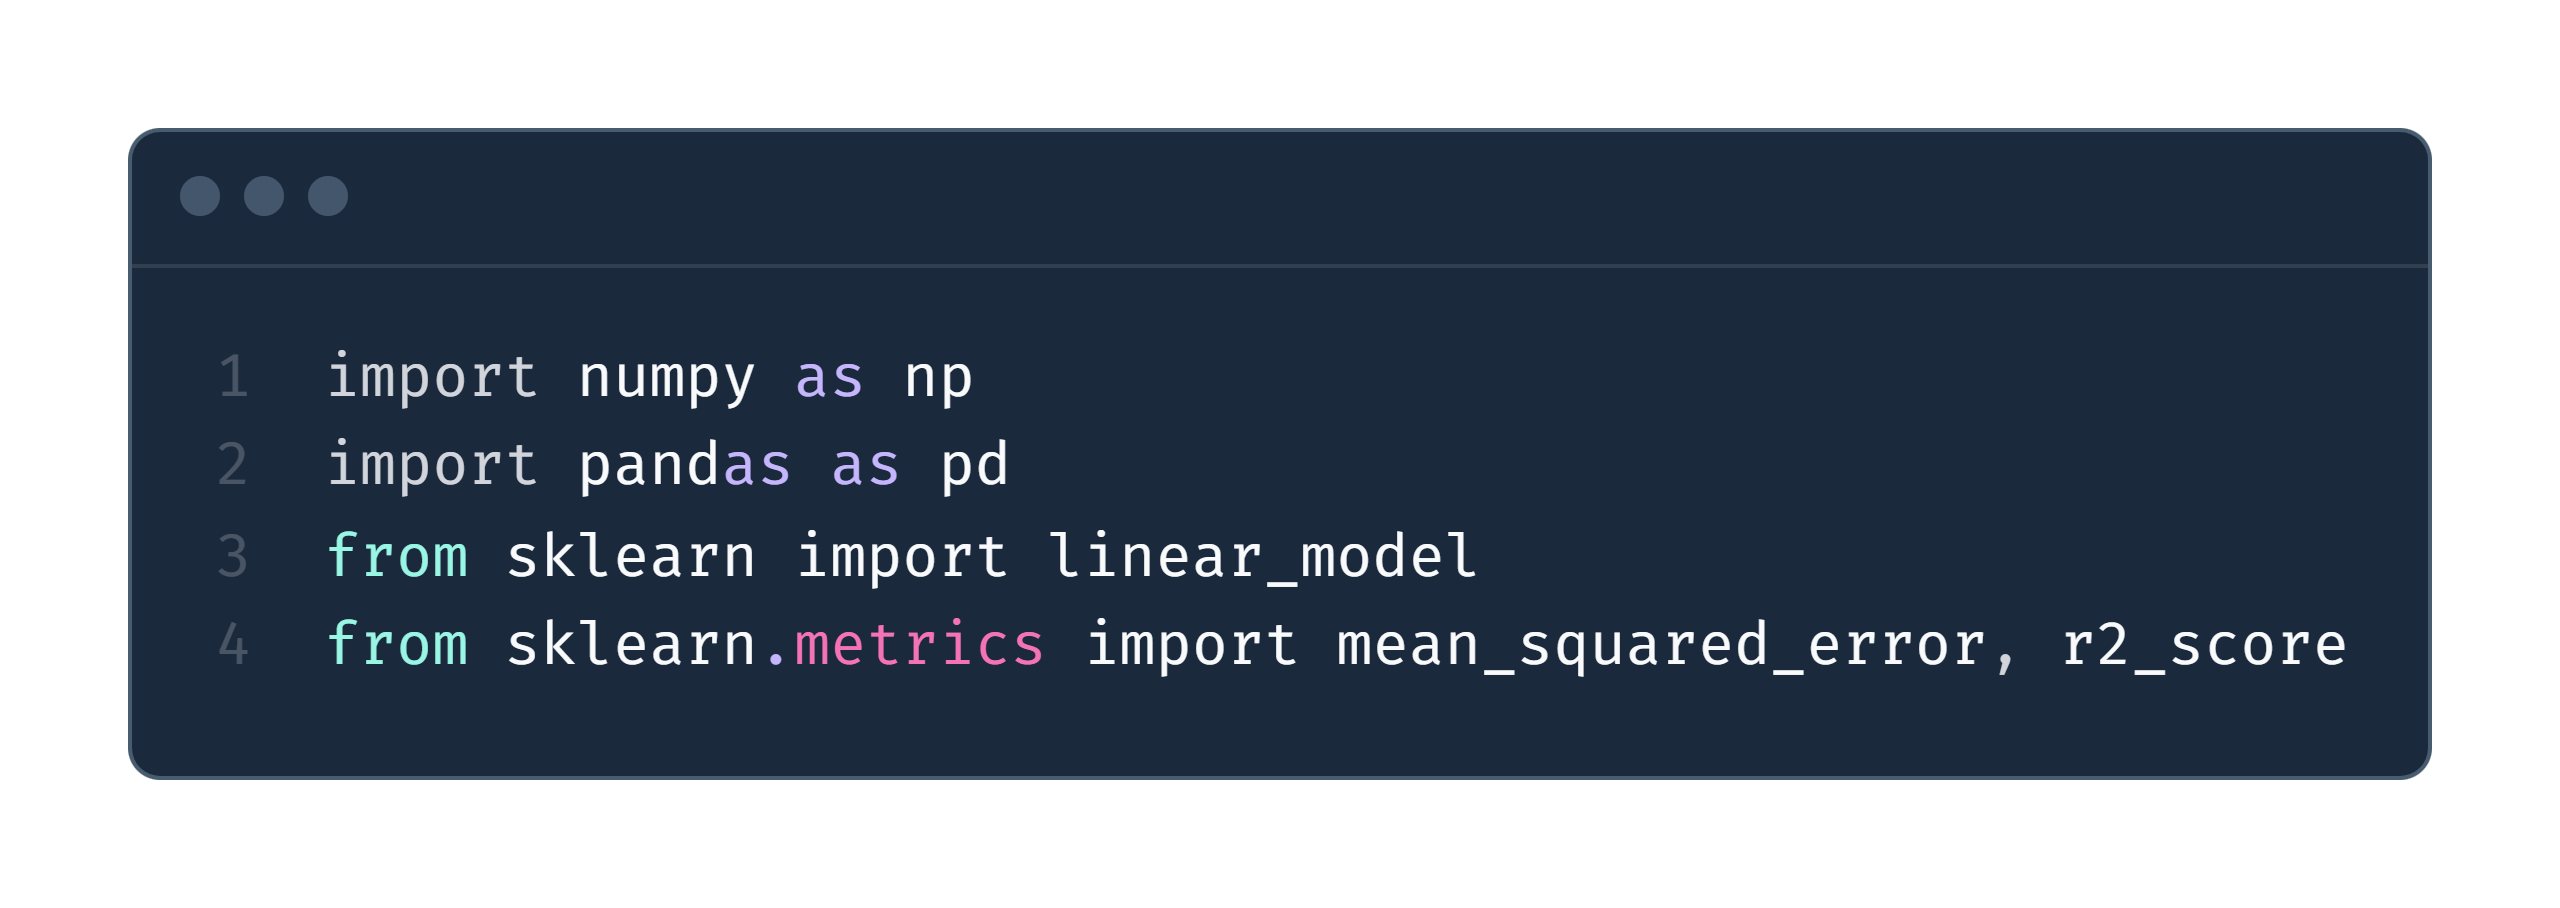
\includegraphics[width=0.5\linewidth]{image.png}
\end{figure}

El código restante y que es importante para obtener los datos que deseamos es el siguiente:
\begin{figure}[h]
    \centering
    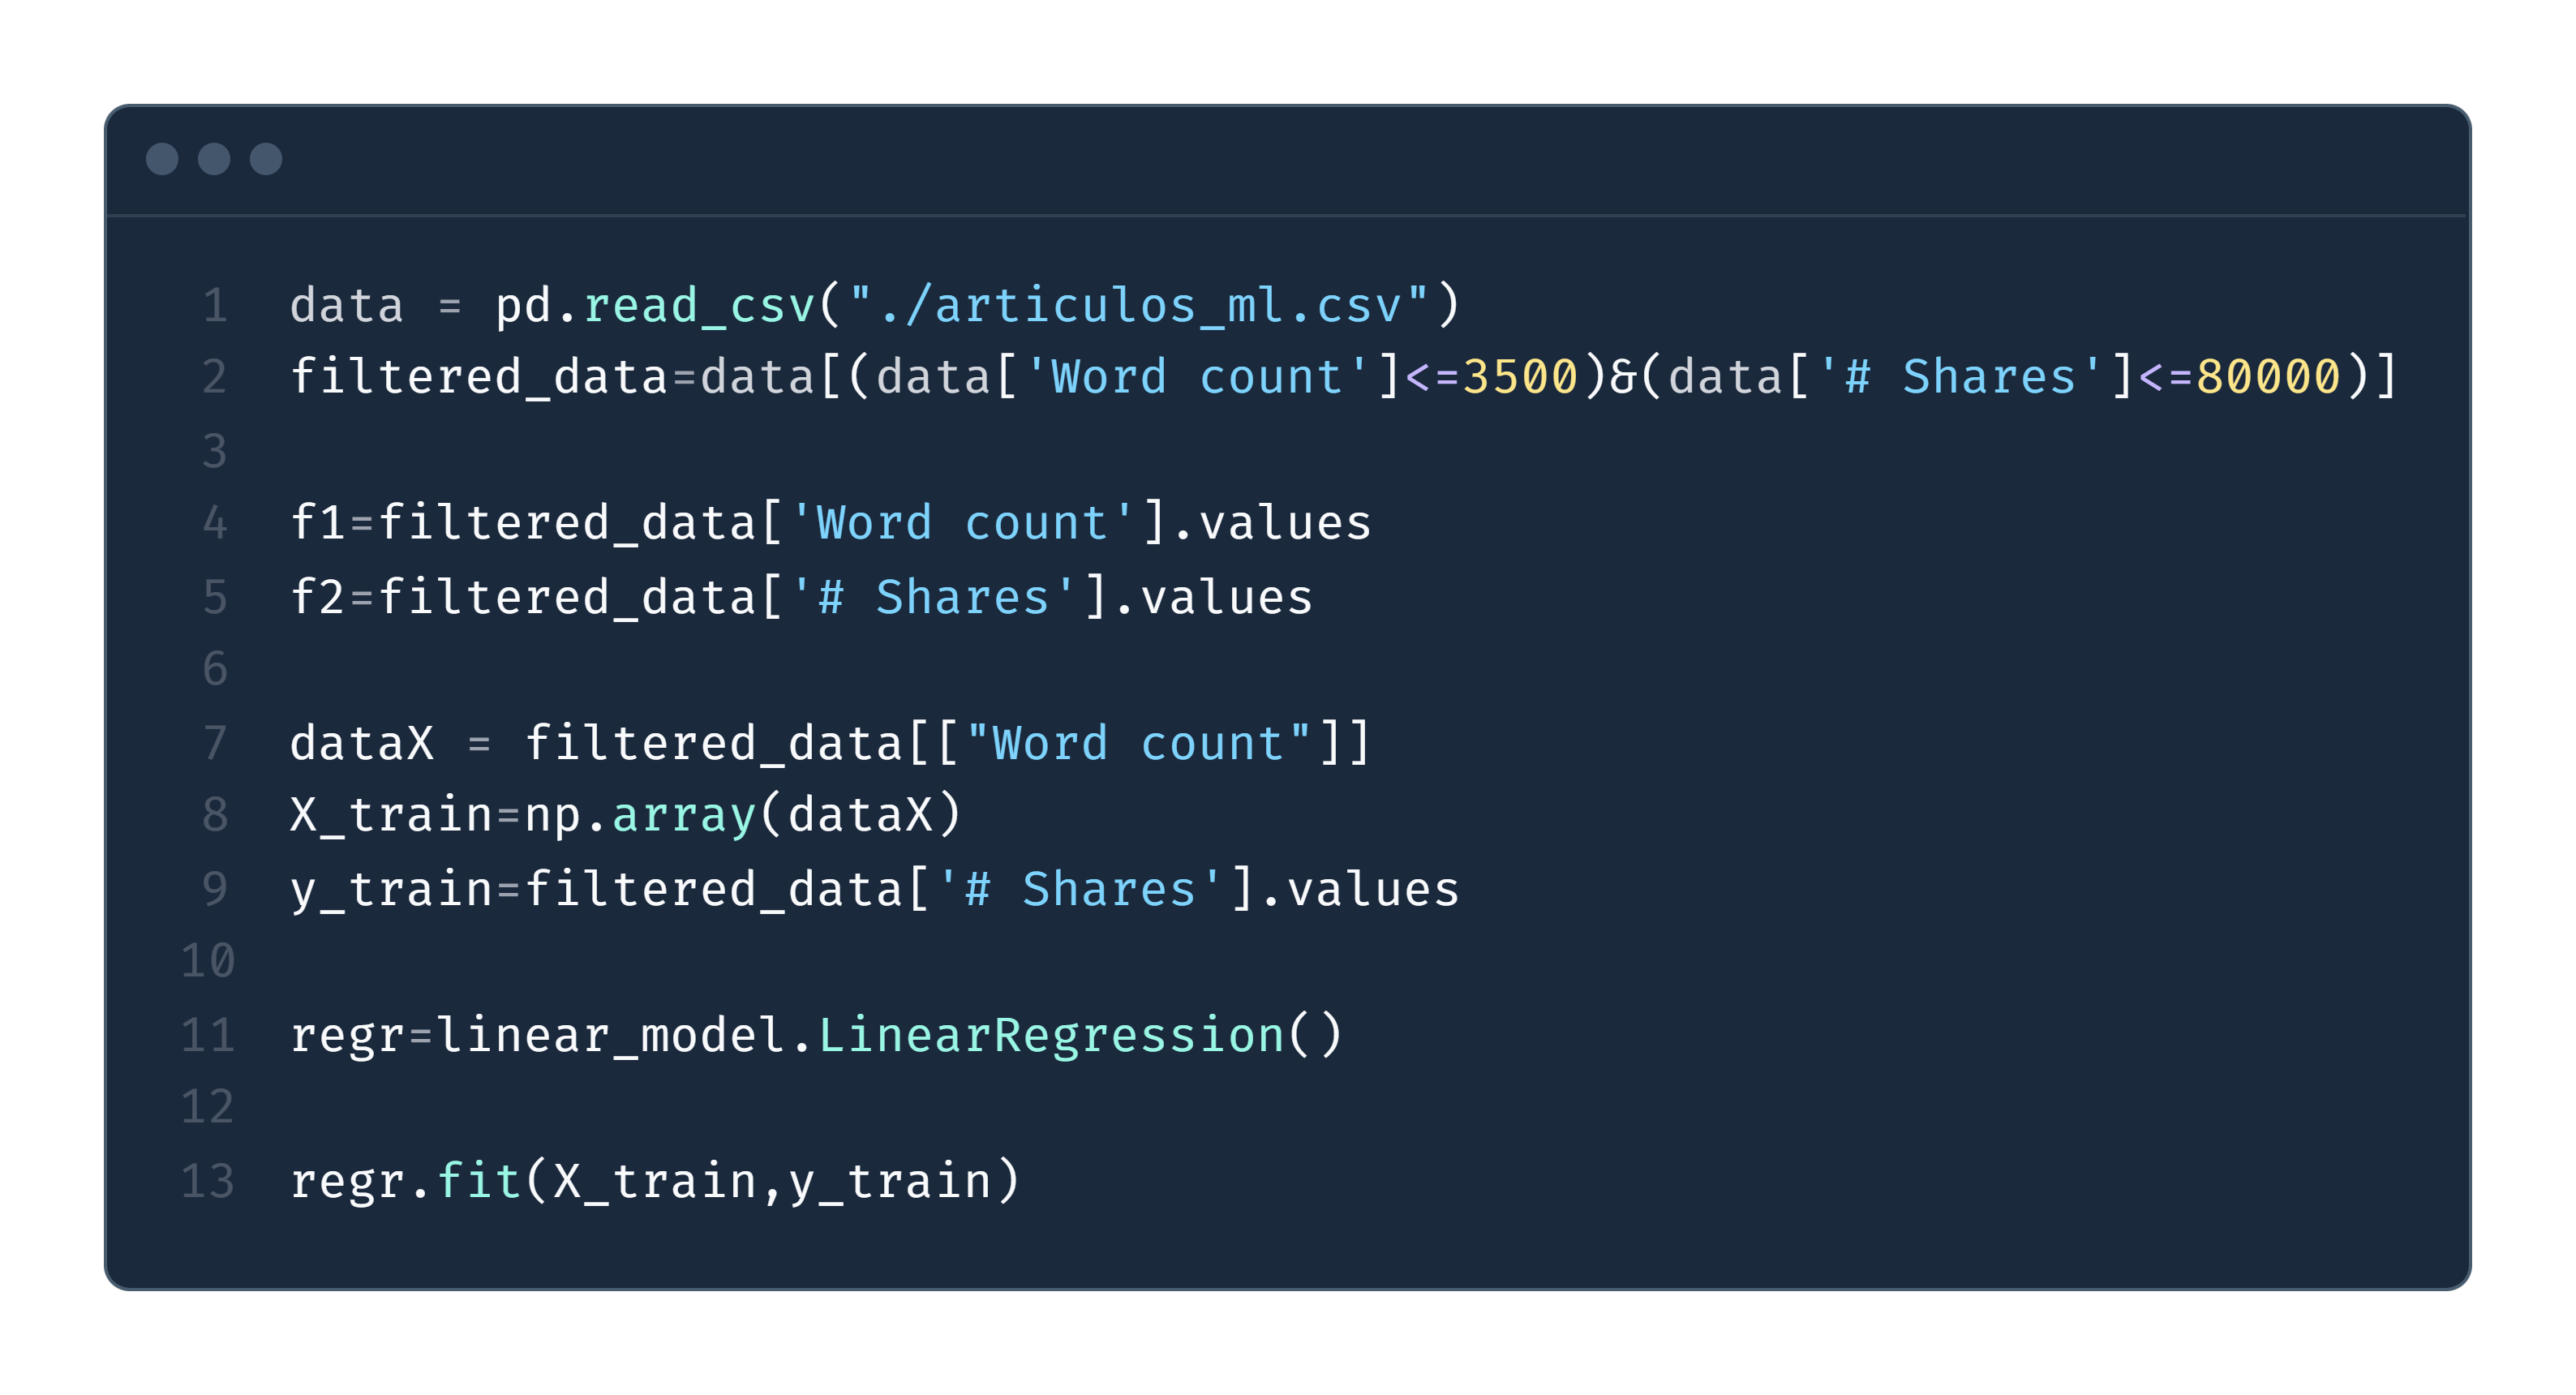
\includegraphics[width=0.75\linewidth]{image_2.png}
\end{figure}

En el código hacemos un filtrado de los datos que obtuvimos del csv, mas específicamente, eliminamos los artículos que tienen una cantidad de palabras mayores a 3500 y los que se hayan compartido mas de 80000 veces. después usando los datos de la cantidad de palabras y el numero de compartidos, se crea y entrena el modelo de regresión lineal.


\section{Resultados}

Al ejecutar el programa obtenemos los siguientes valores

\begin{table}[h]
    \centering
    \begin{tabular}{|c|c|} \hline 
        Coefficients & $5.69765366$ \\ \hline 
        Independent term & $11200.30322307416$\\ \hline 
        Mean squared error & 372888728.34\\ \hline 
        Variance score & 0.06 \\ \hline
    \end{tabular}
    \caption{Caption}
    \label{tab:my_label}
\end{table}


\section{Conclusión}
En base a los datos obtenidos podemos concluir que el modelo de regresión lineal no es efectivo para predecir el numero de veces que sera compartido basándonos solo en la cantidad de palabras.
Esto lo podemos ver explicando que es cada resultado, veremos los mas relevantes:
El termino independiente es de 12200, esto es el valor predicho de compartidos cuando hay cero palabras, lo cual no tiene sentido, un articulo con cero palabras no puede tener tantos compartidos. 
El error cuadrático medio también es bastante alto, por lo que sera normal que el modelo cometa muchos errores en predicciones.

\end{document}